\documentclass[aspectratio=169]{beamer}
\usetheme{Madrid}
\usecolortheme{seahorse}
\usepackage[utf8]{inputenc}
\usepackage{graphicx}
\usepackage{booktabs}
\usepackage{xcolor}
\usepackage{listings}
\usepackage{tikz}

\definecolor{navy}{HTML}{003875}
\definecolor{skyblue}{HTML}{378ADD}
\definecolor{codebg}{rgb}{0.95,0.95,0.92}

\setbeamercolor{palette primary}{bg=navy,fg=white}
\setbeamercolor{palette secondary}{bg=skyblue,fg=white}
\setbeamercolor{palette tertiary}{bg=navy,fg=white}
\setbeamercolor{frametitle}{bg=navy,fg=white}
\setbeamercolor{title}{fg=navy}
\setbeamercolor{block title}{bg=navy,fg=white}

\lstset{
  backgroundcolor=\color{codebg},
  basicstyle=\ttfamily\tiny,
  breaklines=true,
  keywordstyle=\color{navy}\bfseries,
  commentstyle=\color{gray},
  stringstyle=\color{codepurple},
  numbers=left,
  numberstyle=\tiny\color{gray},
  frame=single
}

\title[AI Job Market Intelligence]{\textbf{AI Job Market Intelligence}}
\subtitle{Salaries, Roles \& Global Hiring Trends (2020--2025)}
\author{Muhammad Nouman Hafeez (I210416) \\ M. Asim (I210852) \\ Sara Jabeen (I210624)}
\institute{CS3012 -- Fundamentals of Data Visualization \\ FAST-NUCES Islamabad \\ Instructor: Dr. Atif Mughees}
\date{Spring 2026}

\begin{document}

% ============== SLIDE 1: TITLE ==============
\begin{frame}
\titlepage
\end{frame}

% ============== SLIDE 2: OUTLINE ==============
\begin{frame}{Outline}
\tableofcontents
\end{frame}

% ============== SECTION 1 ==============
\section{Introduction}

\begin{frame}{Project Overview}
\begin{columns}
\column{0.55\textwidth}
\begin{itemize}
    \item \textbf{Course:} CS3012 -- Data Visualization
    \item \textbf{Tool:} Tableau Interactive Dashboard
    \item \textbf{Dataset:} 147,348 real salary submissions
    \item \textbf{Source:} aijobs.net / foorilla.com (CC0 License)
    \item \textbf{Period:} 2022 -- 2025
    \item \textbf{Countries:} 87
\end{itemize}
\column{0.45\textwidth}
\begin{block}{Research Questions}
\footnotesize
\begin{enumerate}
    \item Which AI roles pay the most?
    \item How does salary grow by experience?
    \item How has remote work changed?
    \item Which countries lead AI hiring?
    \item What does salary distribution look like?
\end{enumerate}
\end{block}
\end{columns}
\end{frame}

% ============== SECTION 2 ==============
\section{Dataset}

\begin{frame}{Dataset Description}
\begin{columns}
\column{0.5\textwidth}
\begin{table}
\centering\footnotesize
\begin{tabular}{ll}
\toprule
\textbf{Property} & \textbf{Value} \\
\midrule
Source & aijobs.net \\
Raw Rows & 151,445 \\
Clean Rows & 147,348 \\
Columns (final) & 27 \\
Salary Range & \$37,974--\$385,000 \\
Median Salary & \$147,000 \\
Mean Salary & \$156,237 \\
Unique Titles & 406 \\
License & CC0 Public Domain \\
\bottomrule
\end{tabular}
\end{table}
\column{0.5\textwidth}
\begin{block}{Why This Data Is Real}
\footnotesize
\begin{itemize}
    \item Published by \textbf{aijobs} official Kaggle account
    \item Right-skewed distribution (skewness = 1.35)
    \item US dominates at 90\% (realistic labor market)
    \item 406 raw title variants (not synthetic)
    \item 99.4\% Full-Time entries
\end{itemize}
\end{block}
\end{columns}
\end{frame}

\begin{frame}{Raw Columns (11 Original Fields)}
\footnotesize
\begin{table}
\centering
\begin{tabular}{clll}
\toprule
\textbf{\#} & \textbf{Column} & \textbf{Type} & \textbf{Role} \\
\midrule
1 & work\_year & int & Time axis \\
2 & experience\_level & str & EN/MI/SE/EX \\
3 & employment\_type & str & FT only after cleaning \\
4 & job\_title & str & 406 unique raw titles \\
5 & salary & int & Local currency \\
6 & salary\_currency & str & Currency code \\
7 & salary\_in\_usd & int & \textbf{Primary measure} \\
8 & employee\_residence & str & Worker country \\
9 & remote\_ratio & int & 0 / 50 / 100 \\
10 & company\_location & str & ISO country code \\
11 & company\_size & str & S / M / L \\
\bottomrule
\end{tabular}
\end{table}
\end{frame}

% ============== SECTION 3 ==============
\section{Preprocessing Pipeline}

\begin{frame}{Pipeline Overview (5 Scripts)}
\begin{center}
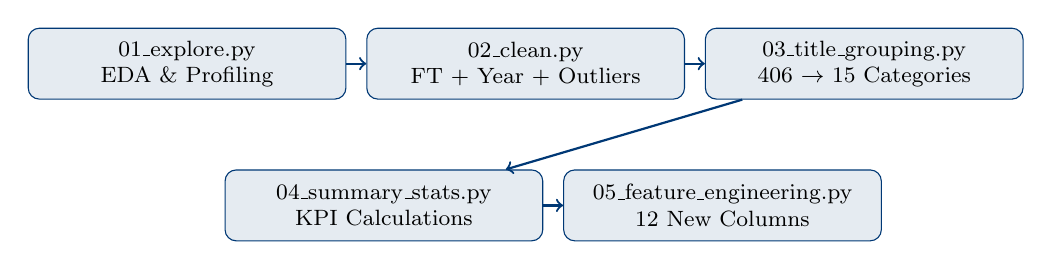
\begin{tikzpicture}[node distance=1.8cm, auto,
    block/.style={rectangle, draw=navy, fill=navy!10, text width=3.8cm, text centered, rounded corners, minimum height=0.9cm, font=\footnotesize}]
    \node[block] (s1) {01\_explore.py\\EDA \& Profiling};
    \node[block, right of=s1, xshift=2.5cm] (s2) {02\_clean.py\\FT + Year + Outliers};
    \node[block, right of=s2, xshift=2.5cm] (s3) {03\_title\_grouping.py\\406 $\rightarrow$ 15 Categories};
    \node[block, below of=s1, xshift=2.5cm] (s4) {04\_summary\_stats.py\\KPI Calculations};
    \node[block, right of=s4, xshift=2.5cm] (s5) {05\_feature\_engineering.py\\12 New Columns};
    \draw[->, thick, navy] (s1) -- (s2);
    \draw[->, thick, navy] (s2) -- (s3);
    \draw[->, thick, navy] (s3) -- (s4);
    \draw[->, thick, navy] (s4) -- (s5);
\end{tikzpicture}
\end{center}
\end{frame}

\begin{frame}{Stage 1 -- Data Cleaning (02\_clean.py)}
\begin{table}
\centering
\begin{tabular}{llrrr}
\toprule
\textbf{Step} & \textbf{Action} & \textbf{Before} & \textbf{After} & \textbf{Removed} \\
\midrule
1 & Keep Full-Time only & 151,445 & 150,541 & 904 \\
2 & Keep 2022--2025 & 150,541 & 150,264 & 277 \\
3 & Remove outliers (P1--P99) & 150,264 & 147,348 & 2,916 \\
\bottomrule
\end{tabular}
\end{table}
\vspace{0.3cm}
\begin{block}{Outlier Bounds}
Lower: \$37,974 \hfill Upper: \$385,000 \hfill Method: 1st--99th Percentile
\end{block}
\end{frame}

\begin{frame}{Stage 2 -- Title Grouping (03\_title\_grouping.py)}
\begin{columns}
\column{0.55\textwidth}
\footnotesize
\textbf{406 raw titles $\rightarrow$ 15 standard categories} via keyword string matching:
\begin{enumerate}\footnotesize
    \item Data Scientist
    \item Data Engineer
    \item ML Engineer / MLOps
    \item Software Engineer
    \item Data Analyst
    \item AI / ML Researcher
    \item Analytics Engineer
    \item Research Scientist
    \item Manager / Director
    \item Data Architect
    \item Product Manager
    \item Data Governance \& Ops
    \item Consultant / Analyst
    \item Other
\end{enumerate}
\column{0.45\textwidth}
\begin{block}{Label Columns Added}
\footnotesize
\begin{tabular}{ll}
\toprule
\textbf{Column} & \textbf{Maps From} \\
\midrule
title\_group & job\_title \\
work\_mode & remote\_ratio \\
exp\_label & experience\_level \\
size\_label & company\_size \\
\bottomrule
\end{tabular}
\end{block}
\end{columns}
\end{frame}

\begin{frame}{Stage 3 -- Feature Engineering (12 New Columns)}
\footnotesize
\begin{table}
\centering
\begin{tabular}{lll}
\toprule
\textbf{Column} & \textbf{Technique} & \textbf{Dashboard Use} \\
\midrule
salary\_band & pd.cut (6 tiers) & Color by pay tier \\
salary\_quartile & pd.qcut (Q1--Q4) & Distribution charts \\
exp\_order & Dict map (1--4) & Sort axis in Tableau \\
region & Dict lookup (87 ISO) & Regional comparison \\
is\_us & Lambda flag & US vs Rest of World \\
is\_ai\_core & Set membership & AI/ML Core vs Data \& Tech \\
year\_avg\_salary & GroupBy + merge & Reference line \\
salary\_vs\_year\_avg & Subtraction & Dollar gap in tooltip \\
salary\_vs\_year\_avg\_pct & Percentage & Color encode deviation \\
role\_avg\_salary & GroupBy + merge & Reference line per role \\
salary\_vs\_role\_avg & Subtraction & Dollar gap in tooltip \\
salary\_vs\_role\_avg\_pct & Percentage & Green/red color encode \\
\bottomrule
\end{tabular}
\end{table}
\textbf{Final dataset:} 147,348 rows $\times$ 27 columns $\cdot$ 0 missing values
\end{frame}

% ============== SECTION 4 ==============
\section{Analysis \& Key Findings}

\begin{frame}{Key Performance Indicators}
\begin{figure}
    \centering
    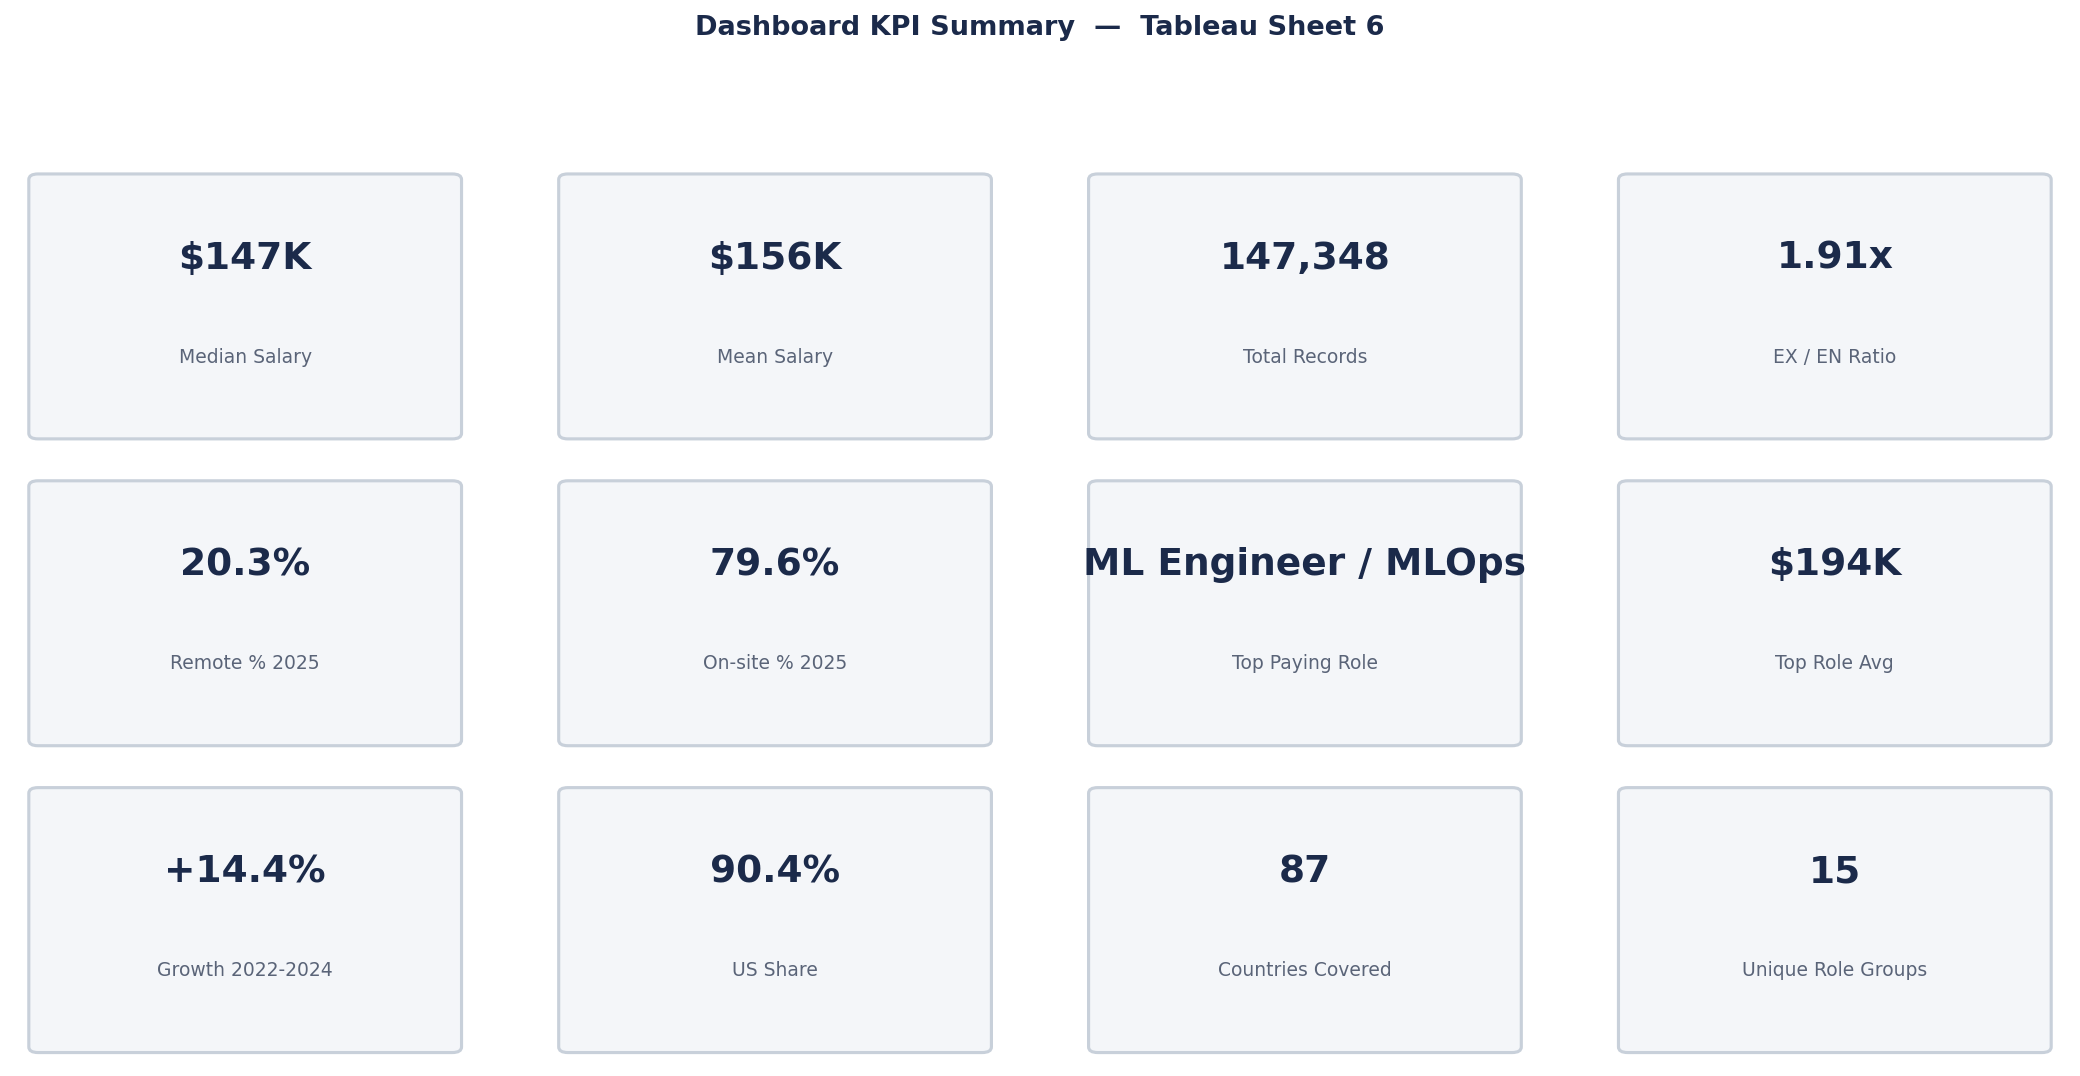
\includegraphics[width=0.85\textwidth]{figures/09_kpi_summary_cards.png}
    \caption{KPI Summary Cards}
\end{figure}
\end{frame}

\begin{frame}{Salary Distribution}
\begin{columns}
\column{0.5\textwidth}
\begin{figure}
    \centering
    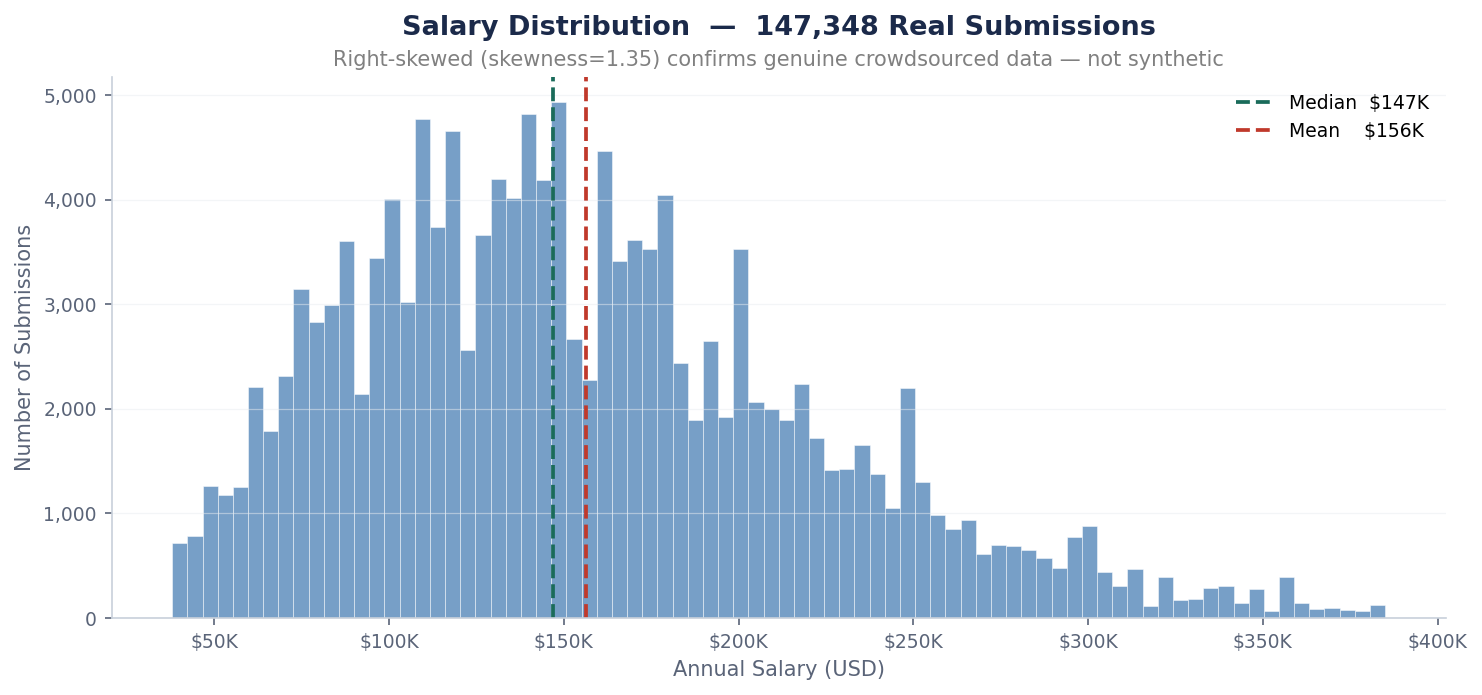
\includegraphics[width=\textwidth]{figures/01_salary_distribution.png}
    \caption{Salary Histogram}
\end{figure}
\column{0.5\textwidth}
\begin{figure}
    \centering
    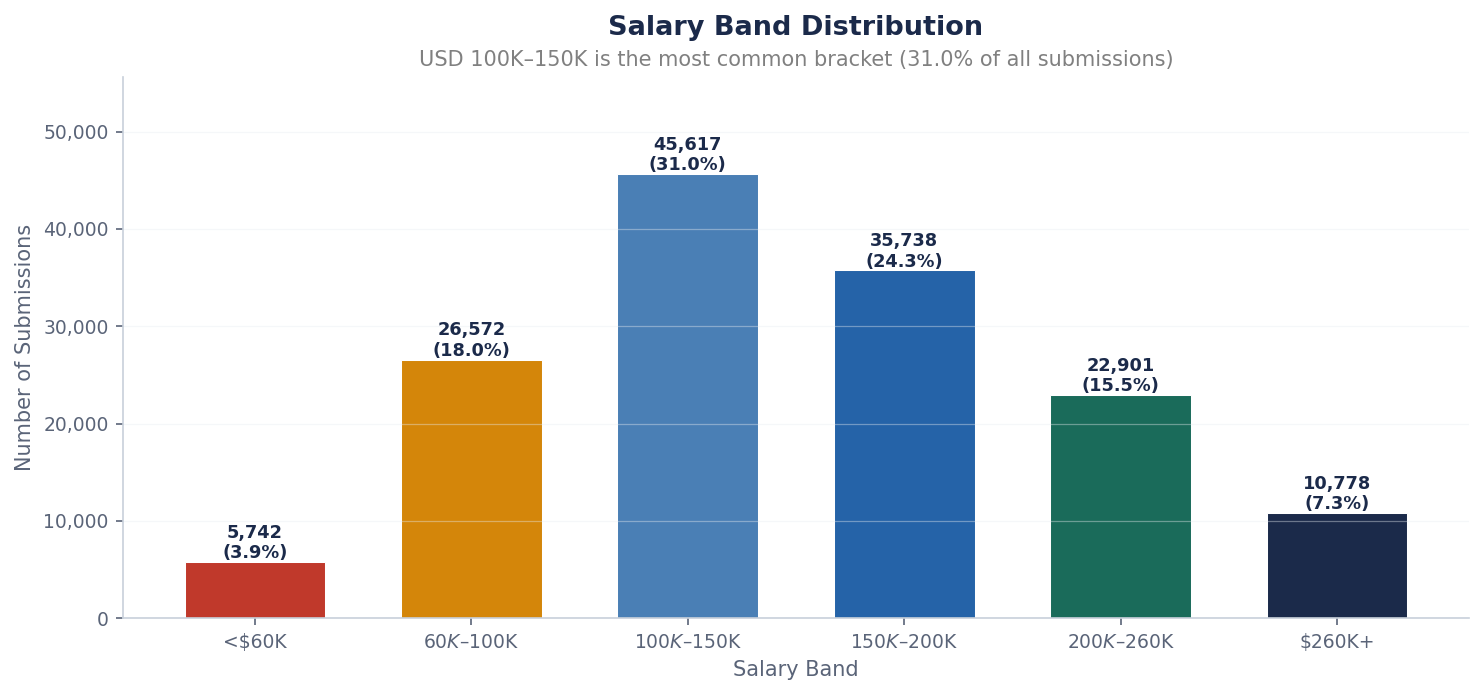
\includegraphics[width=\textwidth]{figures/02_salary_band_distribution.png}
    \caption{Salary Band Distribution}
\end{figure}
\end{columns}
\end{frame}

\begin{frame}{Salary Trends (2022--2025)}
\begin{columns}
\column{0.6\textwidth}
\begin{figure}
    \centering
    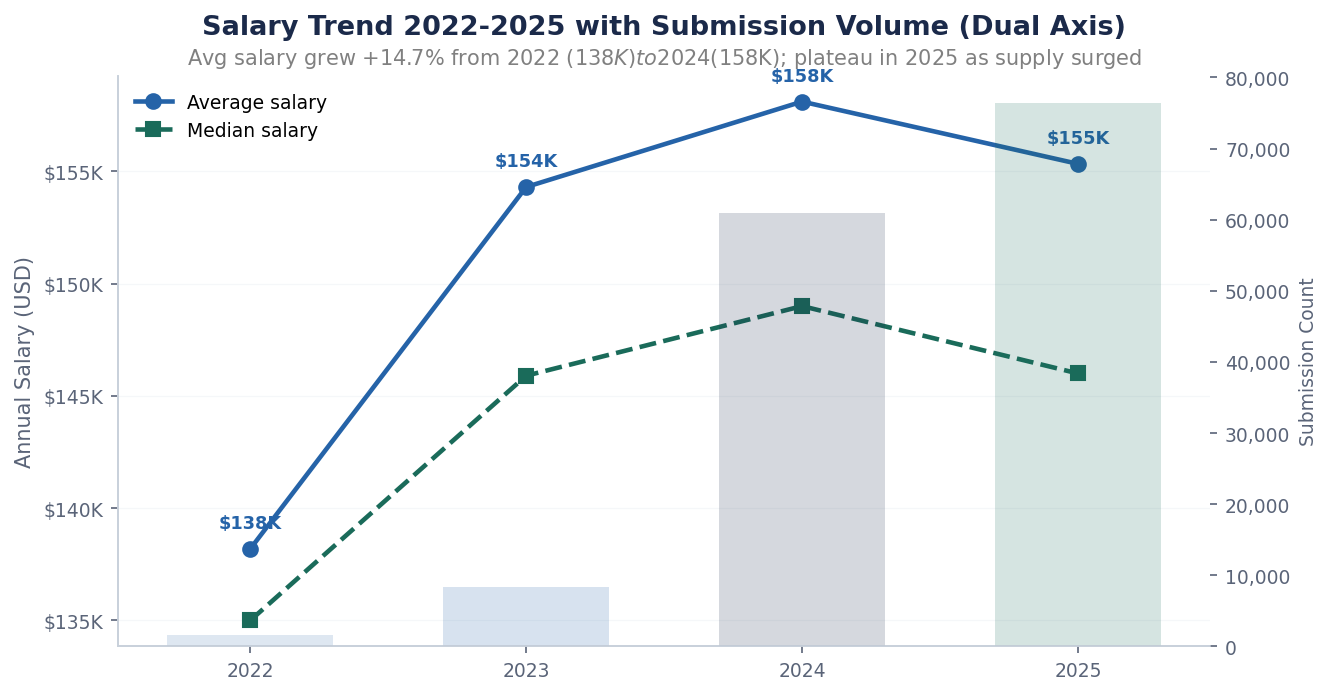
\includegraphics[width=\textwidth]{figures/03_salary_trend_dual_axis.png}
    \caption{Dual-Axis: Avg/Median Salary + Volume}
\end{figure}
\column{0.4\textwidth}
\begin{table}\footnotesize
\centering
\begin{tabular}{lrr}
\toprule
\textbf{Year} & \textbf{Avg} & \textbf{Count} \\
\midrule
2022 & \$138K & 1,587 \\
2023 & \$154K & 8,423 \\
2024 & \$158K & 60,914 \\
2025 & \$155K & 76,424 \\
\bottomrule
\end{tabular}
\end{table}
\begin{alertblock}{Insight}
\footnotesize Median grew 10\% from 2022--2024, then stabilized in 2025.
\end{alertblock}
\end{columns}
\end{frame}

\begin{frame}{Salary by Role}
\begin{figure}
    \centering
    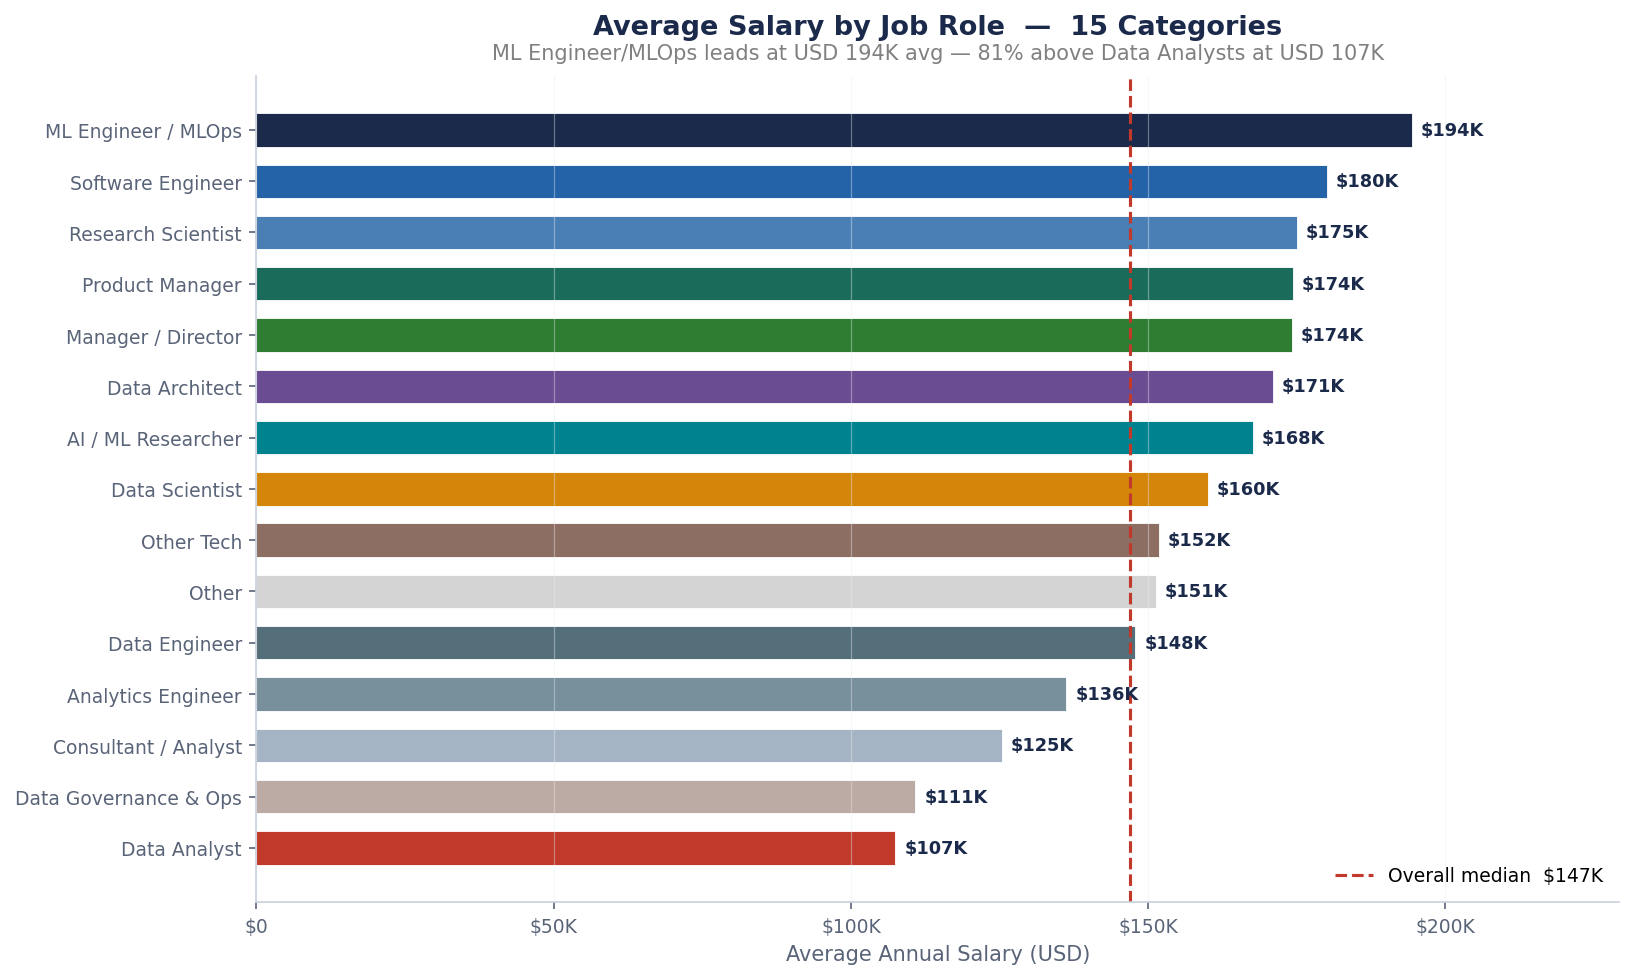
\includegraphics[width=0.75\textwidth]{figures/04_salary_by_role.png}
    \caption{Average Salary by 15 Standardized Role Categories}
\end{figure}
\begin{block}{Top Finding}
ML Engineer / MLOps tops at \$194,303 avg -- 81\% above Data Analysts.
\end{block}
\end{frame}

\begin{frame}{Salary vs Experience Level}
\begin{columns}
\column{0.55\textwidth}
\begin{figure}
    \centering
    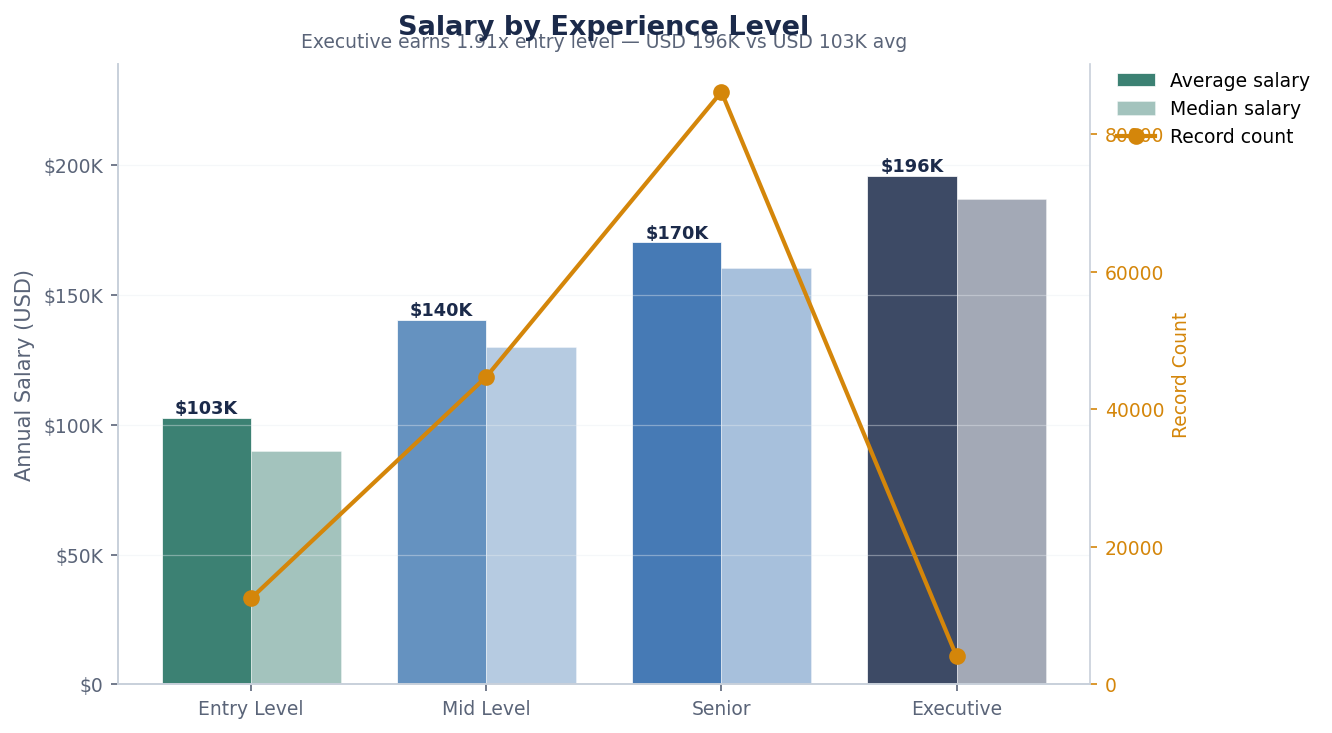
\includegraphics[width=\textwidth]{figures/07_salary_vs_experience.png}
    \caption{Salary by Career Level}
\end{figure}
\column{0.45\textwidth}
\begin{figure}
    \centering
    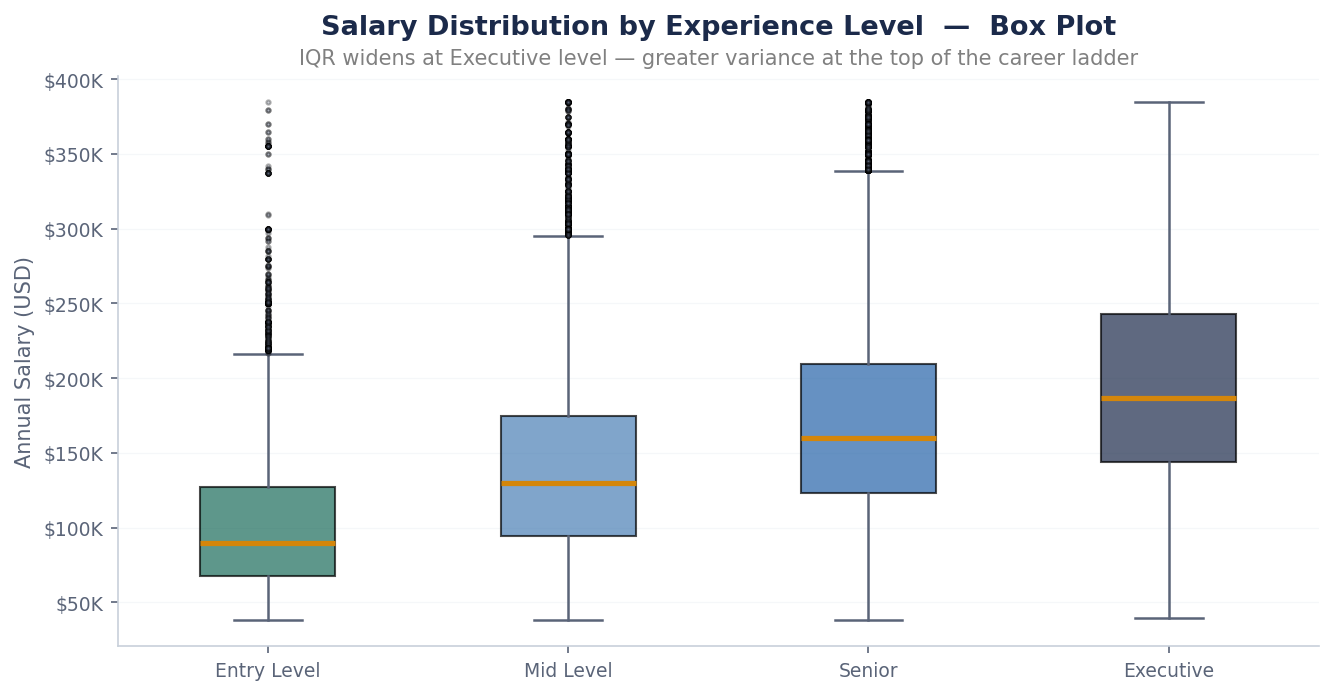
\includegraphics[width=\textwidth]{figures/08_experience_boxplot.png}
    \caption{Experience Level Boxplot}
\end{figure}
\end{columns}
\begin{block}{Key Metric}
Executive earns \textbf{1.91$\times$} Entry Level -- \$195,935 vs \$102,743
\end{block}
\end{frame}

\begin{frame}{Remote Work Collapse}
\begin{columns}
\column{0.5\textwidth}
\begin{figure}
    \centering
    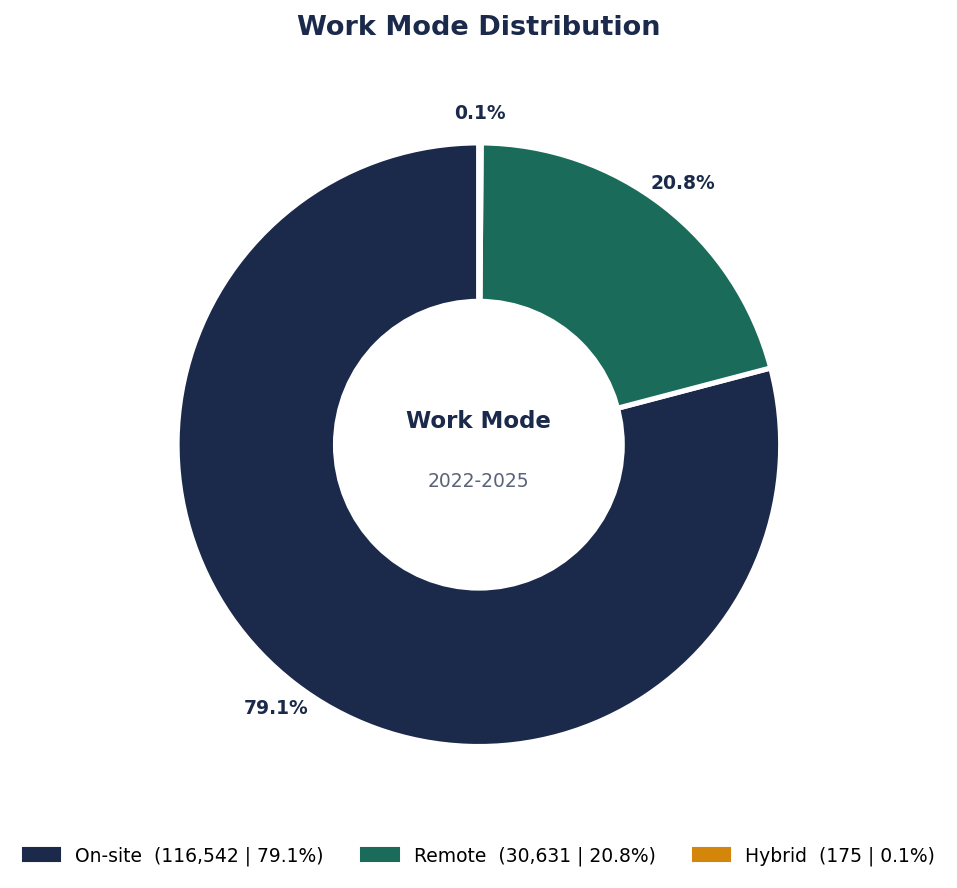
\includegraphics[width=\textwidth]{figures/05_work_mode_donut.png}
    \caption{Work Mode Split (Overall)}
\end{figure}
\column{0.5\textwidth}
\begin{figure}
    \centering
    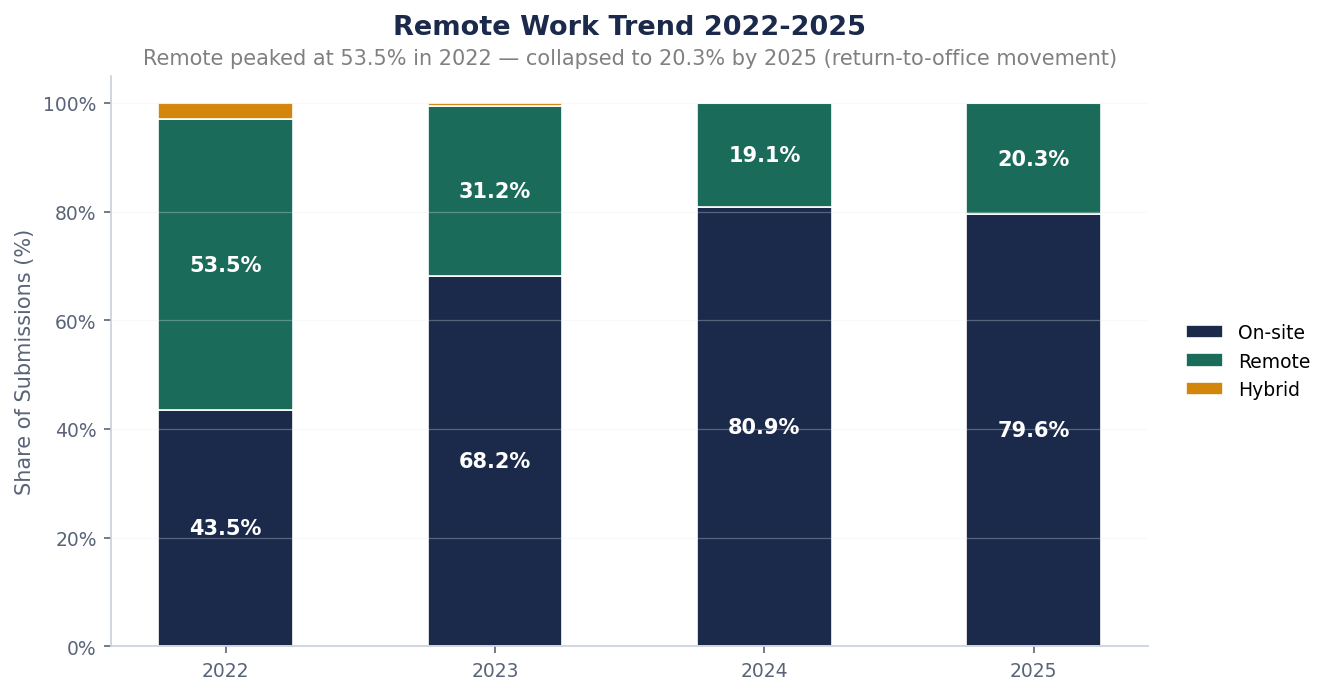
\includegraphics[width=\textwidth]{figures/10_remote_trend_stacked.png}
    \caption{Remote Trend by Year}
\end{figure}
\end{columns}
\begin{alertblock}{Major Finding}
Remote work fell from \textbf{53.5\%} (2022) to \textbf{20.3\%} (2025). On-site now dominates at 79.6\%.
\end{alertblock}
\end{frame}

\begin{frame}{Geographic Analysis}
\begin{columns}
\column{0.5\textwidth}
\begin{figure}
    \centering
    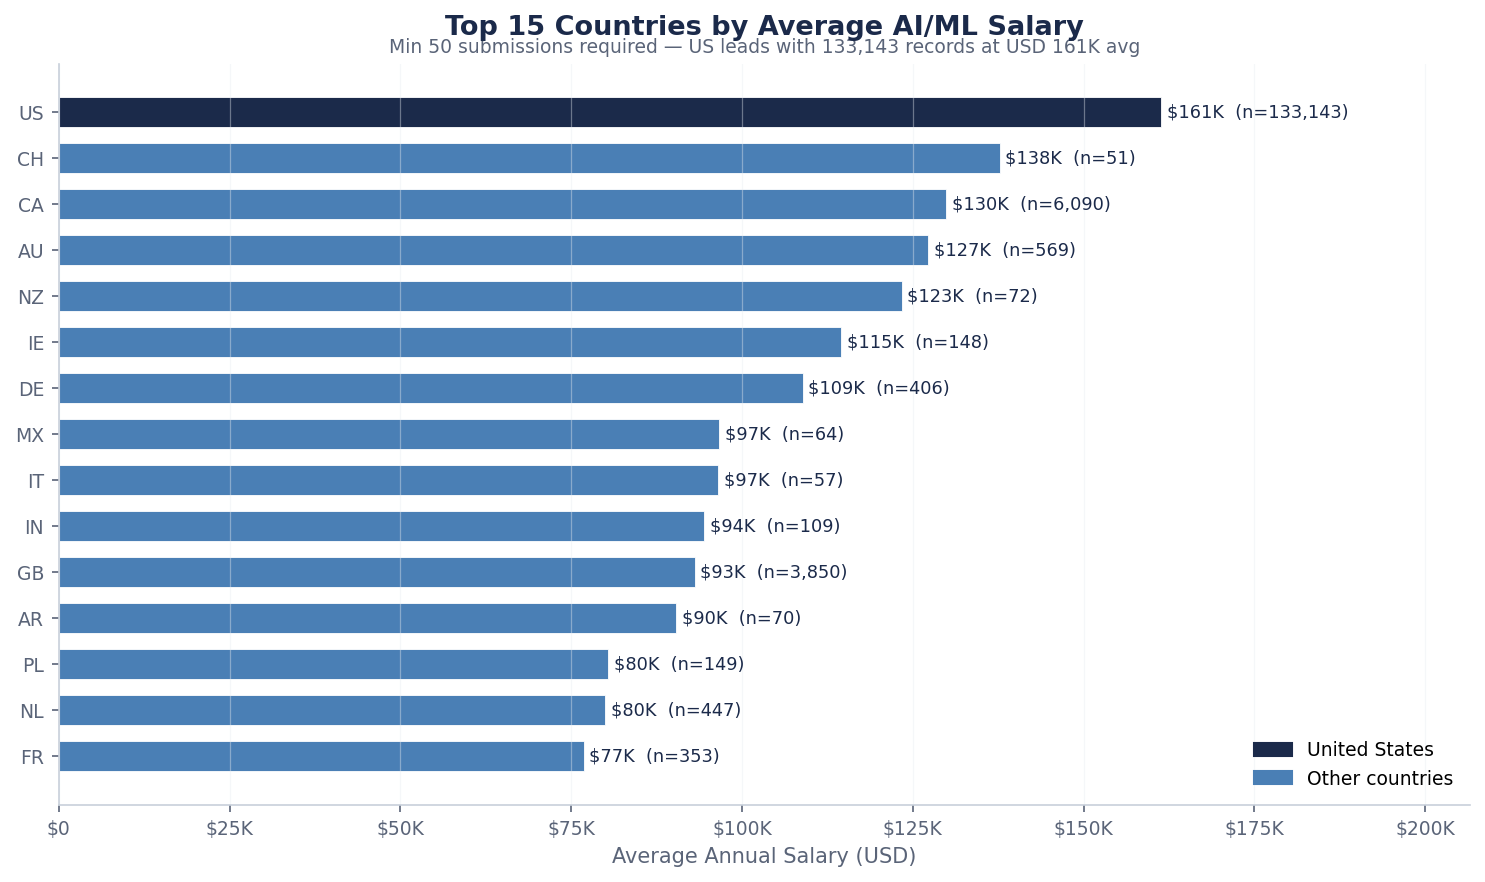
\includegraphics[width=\textwidth]{figures/06_top_countries_salary.png}
    \caption{Top Countries by Salary}
\end{figure}
\column{0.5\textwidth}
\begin{figure}
    \centering
    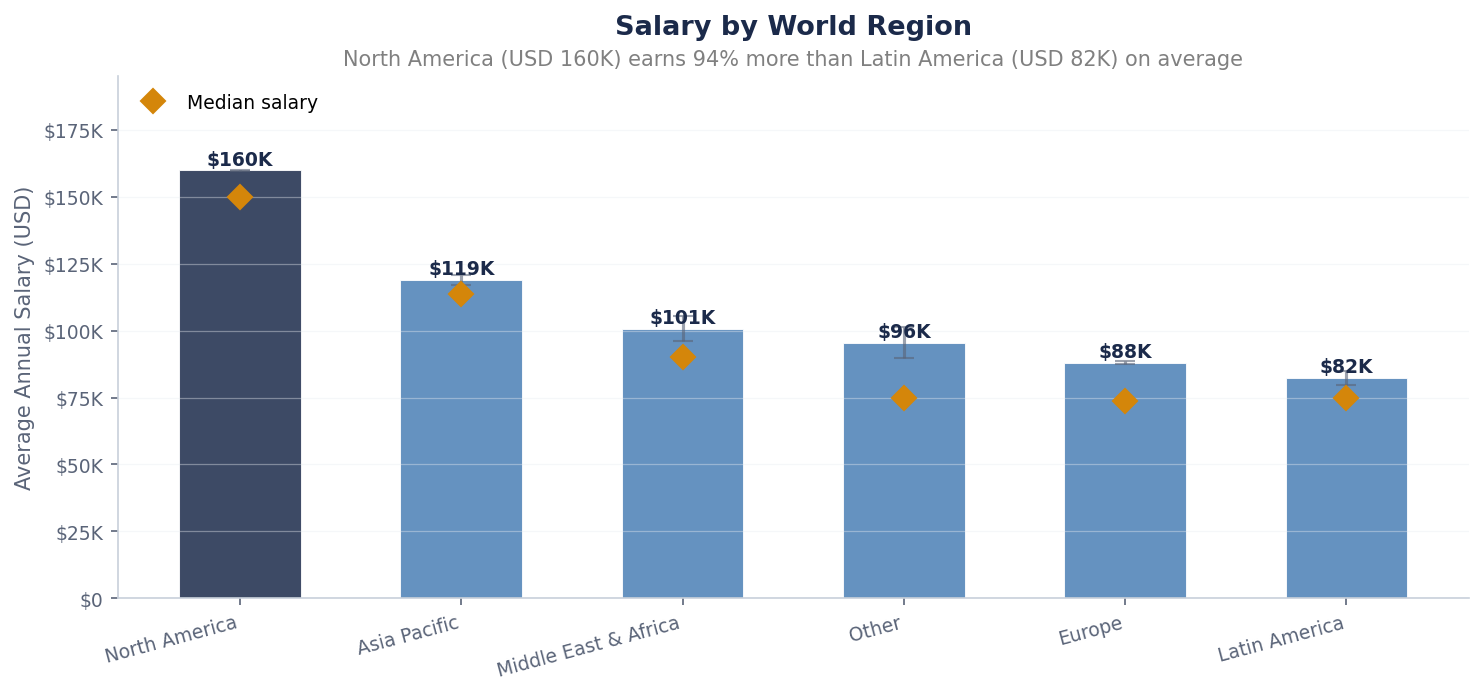
\includegraphics[width=\textwidth]{figures/11_salary_by_region.png}
    \caption{Regional Salary Comparison}
\end{figure}
\end{columns}
\begin{block}{US Dominance}
US: 90.4\% of submissions, \$161,381 avg \hfill Rest of World: \$108,024 avg
\end{block}
\end{frame}

\begin{frame}{US vs Rest of World \& AI Core vs Data/Tech}
\begin{columns}
\column{0.5\textwidth}
\begin{figure}
    \centering
    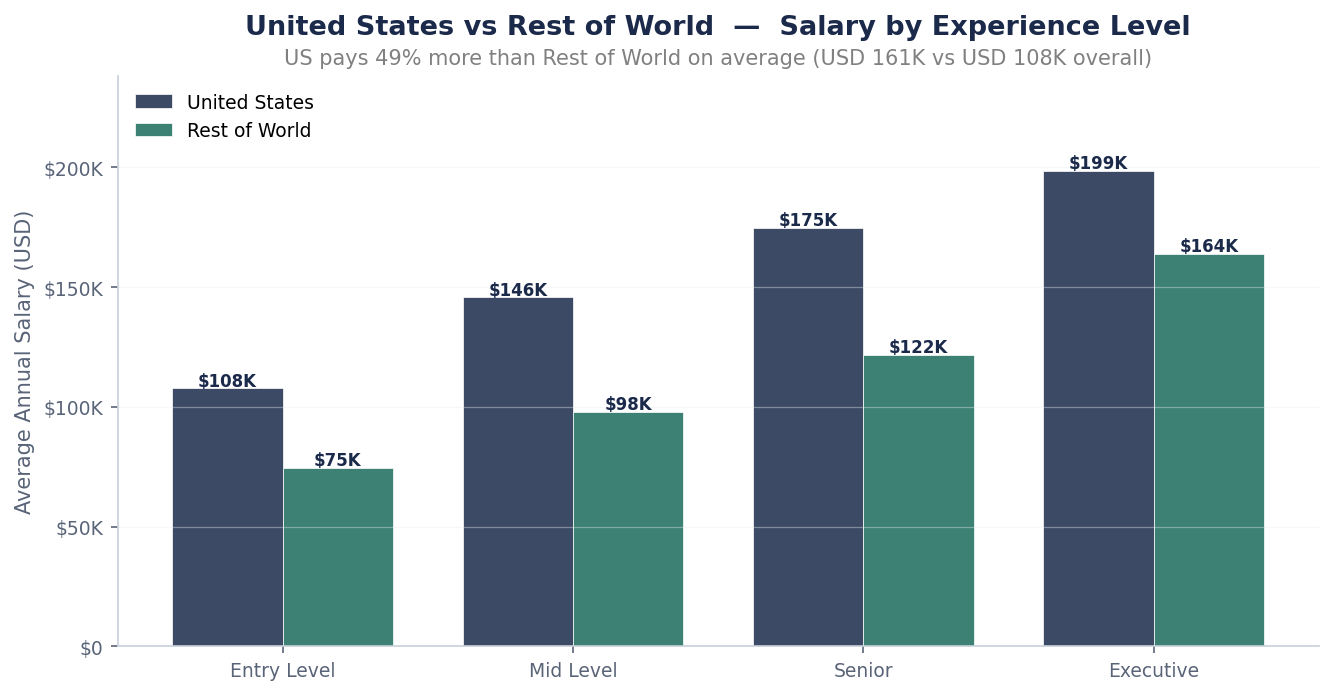
\includegraphics[width=\textwidth]{figures/14_us_vs_row.png}
    \caption{US vs Rest of World}
\end{figure}
\column{0.5\textwidth}
\begin{figure}
    \centering
    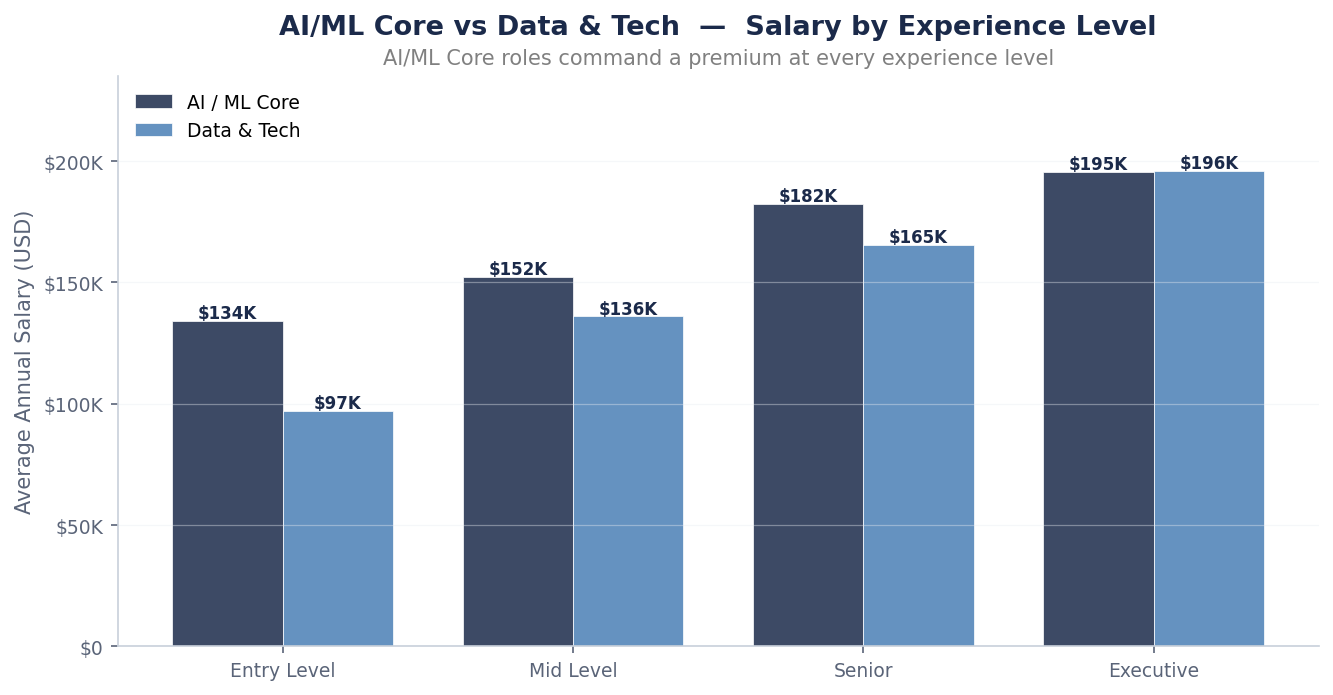
\includegraphics[width=\textwidth]{figures/13_ai_core_vs_data_tech.png}
    \caption{AI/ML Core vs Data \& Tech}
\end{figure}
\end{columns}
\begin{block}{Specialization Premium}
AI/ML Core roles average \$171,009 vs Data \& Tech at \$150,685
\end{block}
\end{frame}

\begin{frame}{Company Size \& Year-Experience Interaction}
\begin{columns}
\column{0.5\textwidth}
\begin{figure}
    \centering
    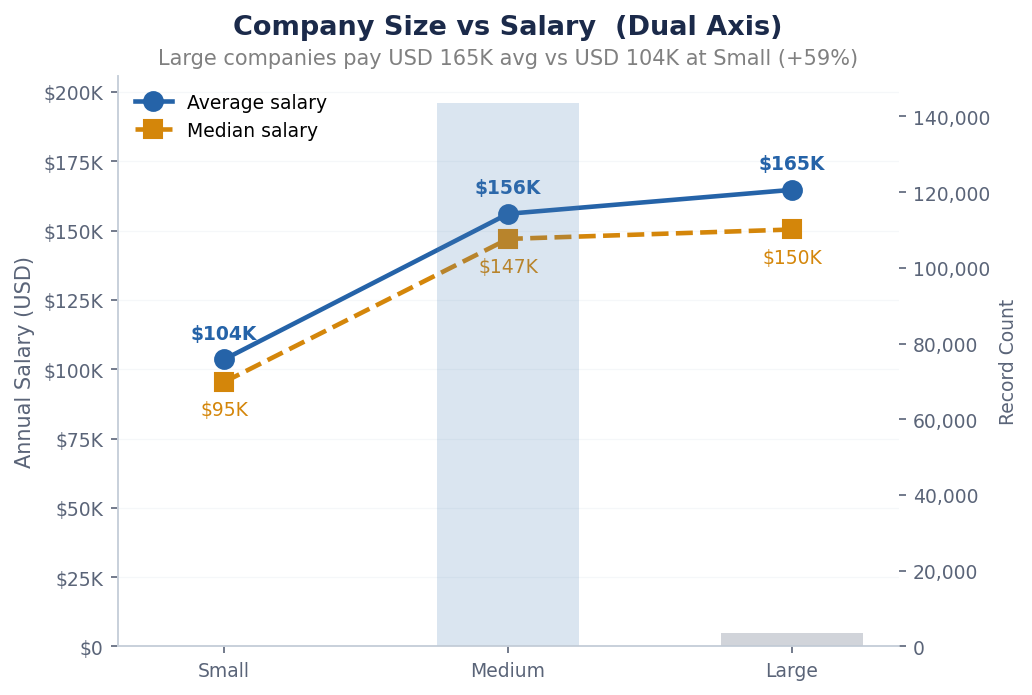
\includegraphics[width=\textwidth]{figures/12_company_size_dual_axis.png}
    \caption{Salary by Company Size}
\end{figure}
\column{0.5\textwidth}
\begin{figure}
    \centering
    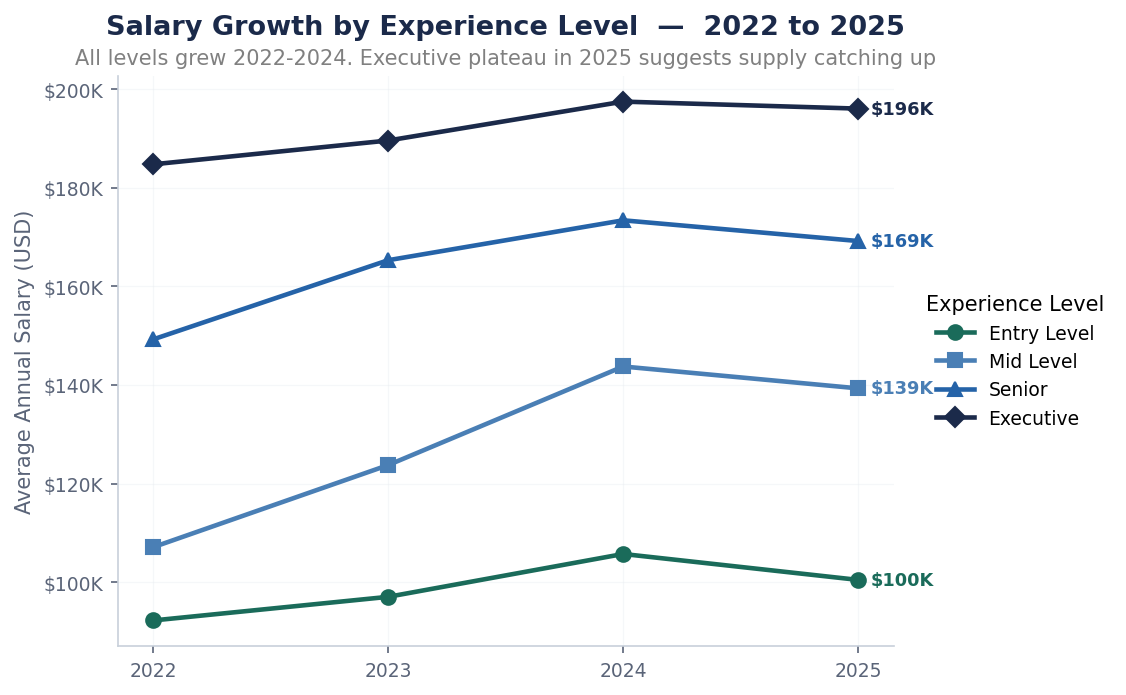
\includegraphics[width=\textwidth]{figures/19_year_experience_lines.png}
    \caption{Year $\times$ Experience Interaction}
\end{figure}
\end{columns}
\end{frame}

\begin{frame}{Advanced Visualizations}
\begin{columns}
\column{0.5\textwidth}
\begin{figure}
    \centering
    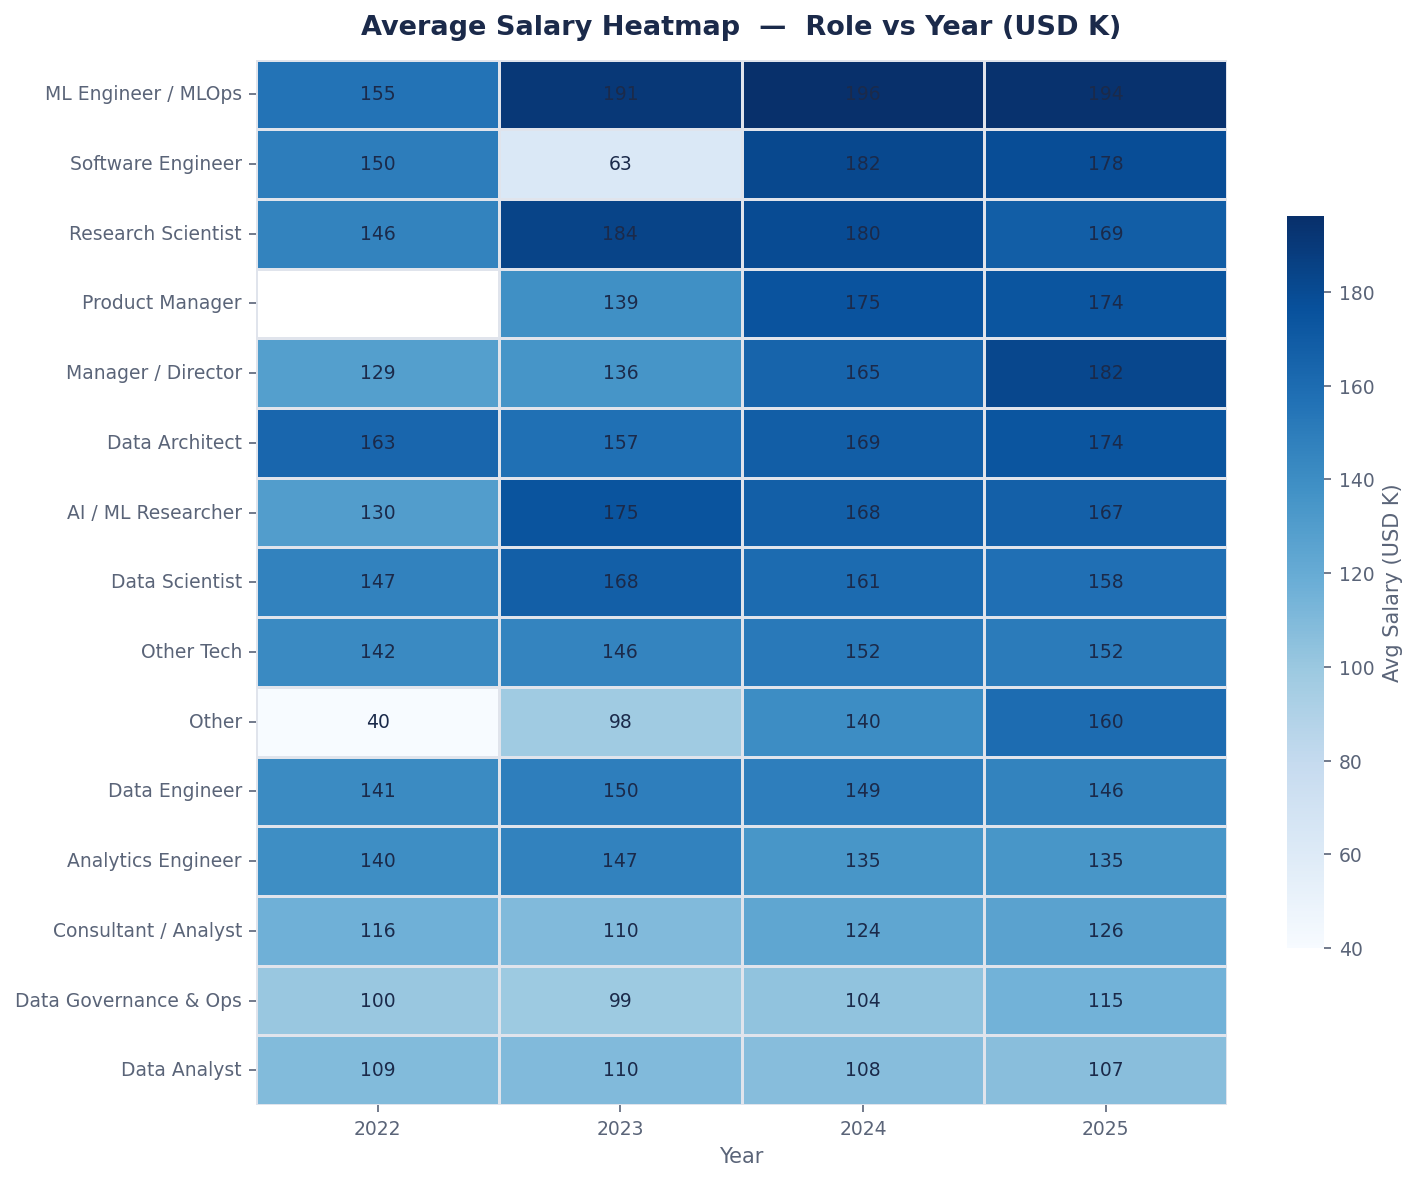
\includegraphics[width=\textwidth]{figures/15_heatmap_role_year.png}
    \caption{Role $\times$ Year Heatmap}
\end{figure}
\column{0.5\textwidth}
\begin{figure}
    \centering
    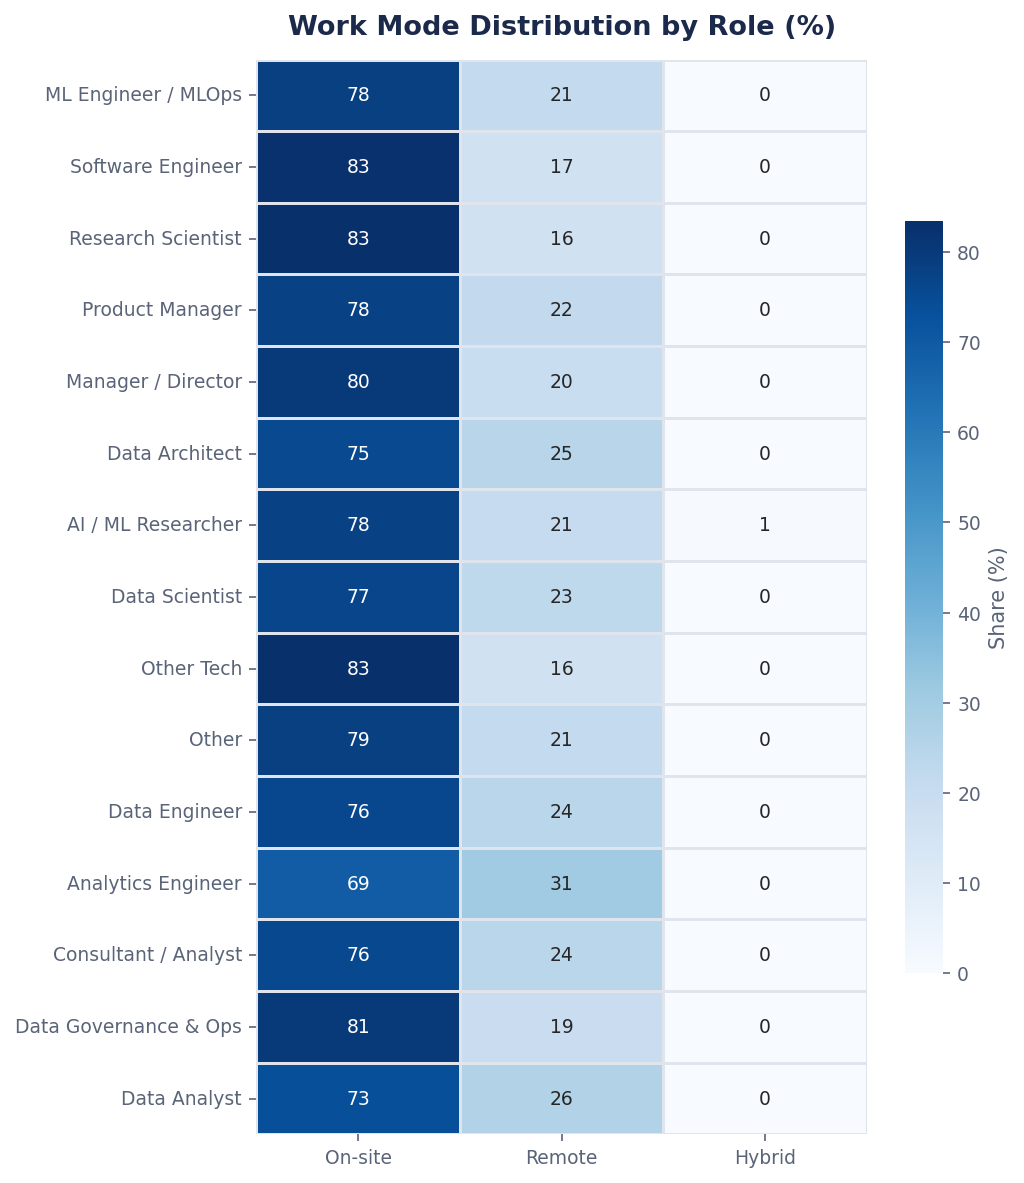
\includegraphics[width=\textwidth]{figures/16_remote_by_role_heatmap.png}
    \caption{Remote \% by Role Heatmap}
\end{figure}
\end{columns}
\end{frame}

\begin{frame}{Quartile \& Range Analysis}
\begin{columns}
\column{0.5\textwidth}
\begin{figure}
    \centering
    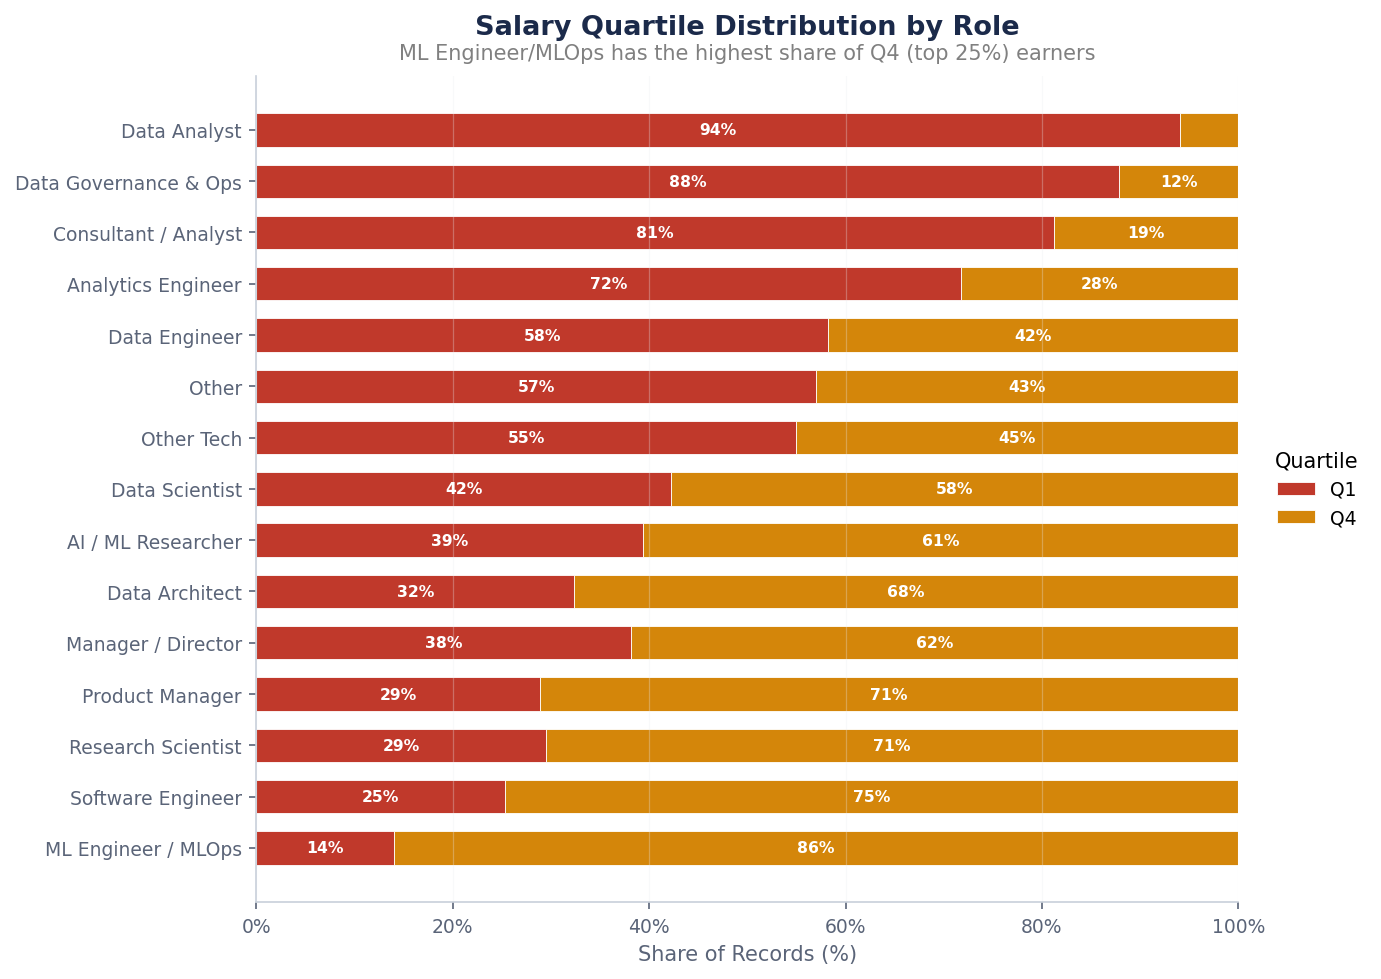
\includegraphics[width=\textwidth]{figures/17_quartile_by_role.png}
    \caption{Salary Quartile by Role}
\end{figure}
\column{0.5\textwidth}
\begin{figure}
    \centering
    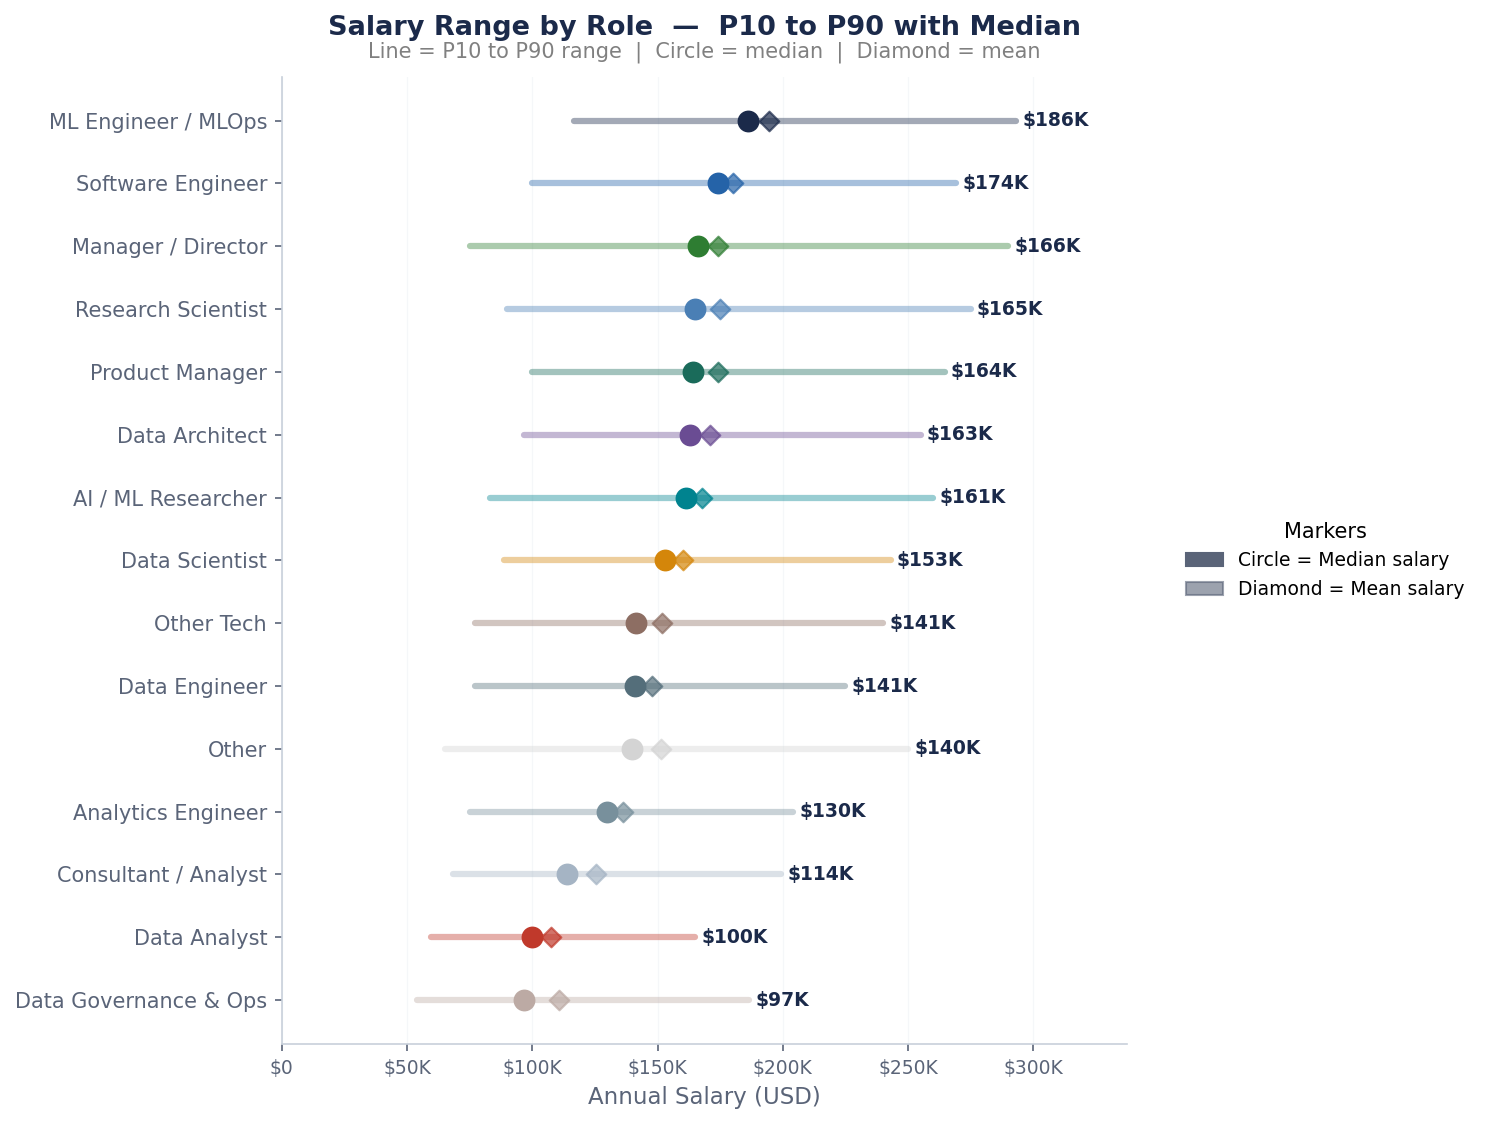
\includegraphics[width=\textwidth]{figures/20_salary_range_by_role.png}
    \caption{Salary Range by Role}
\end{figure}
\end{columns}
\end{frame}

\begin{frame}{Salary vs Year Average (Scatter)}
\begin{figure}
    \centering
    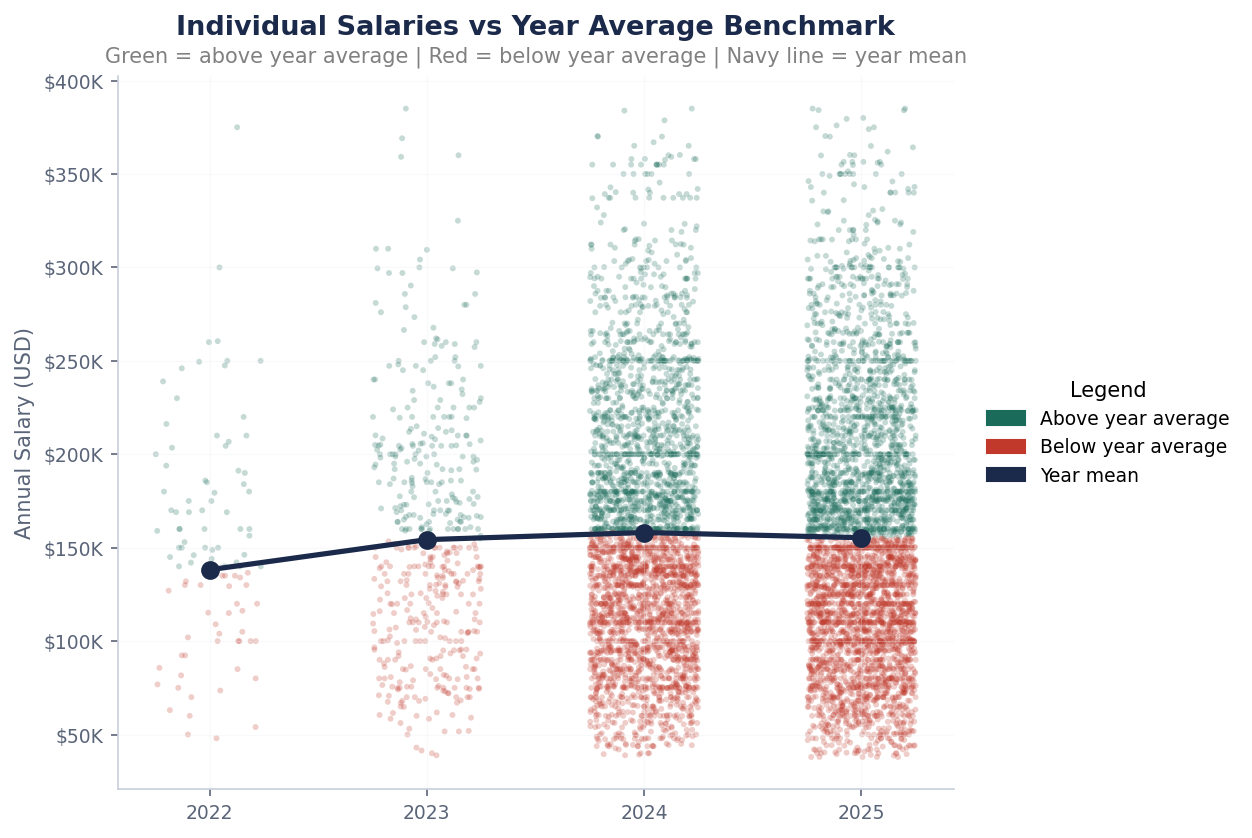
\includegraphics[width=0.7\textwidth]{figures/18_salary_vs_year_avg_scatter.png}
    \caption{Individual Salary Deviation from Year Average}
\end{figure}
\end{frame}

% ============== SECTION 5 ==============
\section{Tableau Dashboard}

\begin{frame}{Dashboard Architecture}
\begin{columns}
\column{0.5\textwidth}
\begin{block}{7 Sheets}
\footnotesize
\begin{enumerate}
    \item Salary Trend (Dual-Axis Line+Bar)
    \item Salary by Role (Horizontal Bar)
    \item Work Mode Split (Donut)
    \item Global Hiring Map (Choropleth)
    \item Salary vs Experience (Bar+Line)
    \item KPI Cards (Text Tiles)
    \item Remote Work Trend (Stacked Bar)
\end{enumerate}
\end{block}
\column{0.5\textwidth}
\begin{block}{Interactive Features}
\footnotesize
\begin{itemize}
    \item \textbf{Dual-axis:} Count bars + salary line
    \item \textbf{Global filters:} Year, Experience, Size
    \item \textbf{Highlight actions:} Cross-sheet linking
    \item \textbf{Parameter toggle:} Top 5 / 10 / All roles
    \item \textbf{5 story annotations}
    \item Canvas: 1200$\times$900 px
\end{itemize}
\end{block}
\end{columns}
\vspace{0.2cm}
\centering
\footnotesize\textbf{Color Theme:} Navy \textcolor{navy}{\rule{0.8cm}{0.3cm}} \#003875 \quad Sky Blue \textcolor{skyblue}{\rule{0.8cm}{0.3cm}} \#378ADD
\end{frame}

\begin{frame}{Calculated Fields in Tableau}
\footnotesize
\begin{table}
\centering
\begin{tabular}{lll}
\toprule
\textbf{Field} & \textbf{Formula} & \textbf{Used On} \\
\midrule
Avg Salary USD & AVG([Salary In Usd]) & All sheets \\
Median Salary USD & MEDIAN([Salary In Usd]) & Sheet 1, 5 \\
EX/EN Ratio & AVG(EX salary) / AVG(EN salary) & KPI Card \\
Remote \% & SUM(IF Remote) / COUNT(*) & KPI Card \\
Role Rank & RANK\_UNIQUE(AVG(salary)) & Sheet 2 \\
Top N Filter & [Role Rank] <= [Parameter] & Sheet 2 \\
\bottomrule
\end{tabular}
\end{table}
\end{frame}

% ============== SECTION 6 ==============
\section{Code Implementation}

\begin{frame}[fragile]{Data Cleaning Code}
\begin{lstlisting}[language=Python]
import pandas as pd
df = pd.read_csv("../data/raw/salaries.csv")

# Step 1: Keep Full-Time only
df_ft = df[df["employment_type"] == "FT"].copy()

# Step 2: Keep 2022-2025
df_yr = df_ft[df_ft["work_year"] >= 2022].copy()

# Step 3: Outlier removal (1st-99th percentile)
q01 = df_yr["salary_in_usd"].quantile(0.01)  # $37,974
q99 = df_yr["salary_in_usd"].quantile(0.99)  # $385,000
df_clean = df_yr[
    (df_yr["salary_in_usd"] >= q01) &
    (df_yr["salary_in_usd"] <= q99)
].copy()

df_clean.to_csv("../data/processed/salaries_clean.csv", index=False)
# Result: 147,348 rows, 11 columns
\end{lstlisting}
\end{frame}

\begin{frame}[fragile]{Title Grouping Code (406 $\rightarrow$ 15)}
\begin{lstlisting}[language=Python]
def group_title(title: str) -> str:
    t = title.lower()
    if any(x in t for x in [
        "data scientist", "data science", "applied scientist"]):
        return "Data Scientist"
    elif any(x in t for x in [
        "machine learning engineer", "ml engineer", "mlops"]):
        return "ML Engineer / MLOps"
    elif any(x in t for x in [
        "data analyst", "bi analyst", "reporting analyst"]):
        return "Data Analyst"
    elif any(x in t for x in [
        "ai engineer", "deep learning", "nlp engineer"]):
        return "AI / ML Researcher"
    # ... 15 total categories
    else:
        return "Other"

df["title_group"] = df["job_title"].apply(group_title)
\end{lstlisting}
\end{frame}

\begin{frame}[fragile]{Feature Engineering Code}
\begin{lstlisting}[language=Python]
# Salary Band (6 tiers)
bins = [0, 60000, 100000, 150000, 200000, 260000, 385001]
labels = ["<$60K","$60K-$100K","$100K-$150K",
          "$150K-$200K","$200K-$260K","$260K+"]
df["salary_band"] = pd.cut(df["salary_in_usd"], bins=bins, labels=labels)

# Salary Quartile
df["salary_quartile"] = pd.qcut(df["salary_in_usd"], q=4,
    labels=["Q1-Bottom 25%","Q2-25-50%","Q3-50-75%","Q4-Top 25%"])

# Region mapping (87 ISO codes -> 6 regions)
region_map = {"US":"North America", "CA":"North America",
              "GB":"Europe", "DE":"Europe", ...}
df["region"] = df["company_location"].map(region_map).fillna("Other")

# Salary vs Year Average
year_avg = df.groupby("work_year")["salary_in_usd"].mean()
df["year_avg_salary"] = df["work_year"].map(year_avg).round(0)
df["salary_vs_year_avg"] = (df["salary_in_usd"] - df["year_avg_salary"])
\end{lstlisting}
\end{frame}

% ============== SECTION 7 ==============
\section{Conclusion}

\begin{frame}{Key Takeaways}
\begin{columns}
\column{0.5\textwidth}
\begin{block}{Market Insights}
\begin{itemize}
    \item Median AI salary: \textbf{\$147,000}
    \item ML Engineer tops at \textbf{\$194K}
    \item Executive-to-Entry ratio: \textbf{1.91$\times$}
    \item Remote work collapsed: 53\% $\rightarrow$ 20\%
    \item US dominates with 90\% of data
\end{itemize}
\end{block}
\column{0.5\textwidth}
\begin{block}{Technical Contributions}
\begin{itemize}
    \item 5-script preprocessing pipeline
    \item 12 engineered analytical columns
    \item 7-sheet interactive Tableau dashboard
    \item 20 analytical visualizations
    \item Zero missing values in final dataset
\end{itemize}
\end{block}
\end{columns}
\vspace{0.3cm}
\begin{alertblock}{Central Data Story}
The AI job market has shifted from a remote-first, high-growth phase (2022) to a stabilized, on-site-dominant market (2025). Specializing in ML Engineering yields the highest returns.
\end{alertblock}
\end{frame}

\begin{frame}{Repository \& Links}
\begin{block}{Project Repository}
\centering
\large \url{https://github.com/noumanic/ai-job-market-analytics}
\end{block}
\vspace{0.3cm}
\footnotesize
\begin{table}
\centering
\begin{tabular}{ll}
\toprule
\textbf{Resource} & \textbf{Location} \\
\midrule
Raw Dataset & data/raw/salaries.csv \\
Enhanced Dataset & data/processed/salaries\_enhanced.csv \\
Preprocessing Scripts & preprocessing/ (5 scripts) \\
Tableau Workbook & tableau/ai\_job\_market\_dashboard.twbx \\
Project Proposal & docs/Group8\_CS3012\_ProjectProposal.pdf \\
Full Report (LaTeX) & docs/Final\_Project\_Report.tex \\
\bottomrule
\end{tabular}
\end{table}
\end{frame}

\begin{frame}
\centering
\Huge \textcolor{navy}{\textbf{Thank You!}} \\
\vspace{0.5cm}
\large Questions? \\
\vspace{1cm}
\footnotesize
Muhammad Nouman Hafeez (I210416) $\cdot$ M. Asim (I210852) $\cdot$ Sara Jabeen (I210624) \\
CS3012 -- FAST-NUCES Islamabad -- Spring 2026
\end{frame}

\end{document}
